%%%%%%%%%%%%%%%%%%%%%%%%%%%%%%%%%%%%%%%%%%%%%%%%%%%%%%%%%%%%%%%%%
\subsection{\RM}		%	TESTFÄLLE - RMed
%%%%%%%%%%%%%%%%%%%%%%%%%%%%%%%%%%%%%%%%%%%%%%%%%%%%%%%%%%%%%%%%%

\noindent
Nun wird eine vergleichbare Analyse für den Algorithmus \RM durchgeführt. Hierbei wird die Güte der Approximation der Theoreme~\ref{theo: med_28} und ~\ref{theo: med_29} aus dem Paper~\cite[S.24]{meyer2} experimentell untersucht.\\[.1cm]
Aufgrund der limitierten Zeit dieser Arbeit und der im direkten Vergleich zu \Rm deutlich höheren Laufzeit, konnte der Datensatz für den Algorithmus \RM nicht so umfangreich ausfallen wie gehofft. Die vorliegende Implementierung erlaubt diesen jedoch nach Bedarf aufzustocken. Wie bei seiner Analyse bereits festgehalten wurde, ist die Auswertung des Algorithmus \RM für eine Eingabemenge $X$ mit einer Mächtigkeit von $n \leq 2^{16}$ uninteressant. Somit wurden für den Parameter $n$ die Werte $n =2^i$, $i\in\{16,\cdots,20\}$ gewählt.\\[.05cm]
Um jedoch ein Gefühl für die Auswirkung der Parameter zu gewinnen wurde zum Test der Parameter $d(n)$ auf die nächst größere beziehungsweise kleinere Ganzzahl gerundet. Bei der Wahl von $n=2^{18}$, $k(n)=2^{12}$ sowie $d_1(n)=2$ und $d_2(n)=3$ halbiert sich, wie in Abbildung~\ref{fig: med_theo28_comp} zu sehen, sowohl die \fg des Median Elements, als auch die Arbeit $w(n)$ bei Auf- und Abrundung zwischen $2$ und $3$. Die \fg aller nicht-Median Elemente \fgr verdoppelt sich hingegen.

% ---------------------------------------------------------------
%	FIG: FG COMP
\begin{figure}[H]
	\hspace*{-1.1cm}
    \begin{minipage}[t]{.30\textwidth}
        \centering
		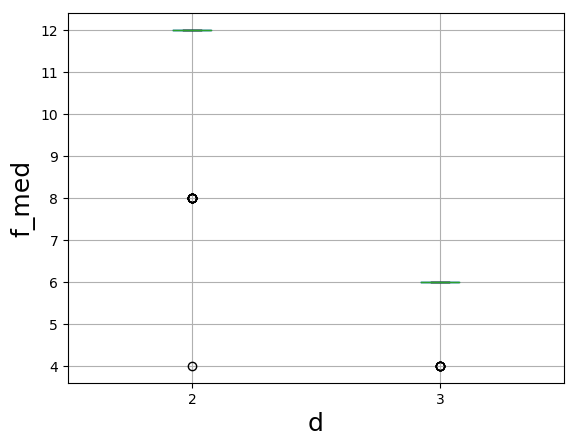
\includegraphics[width=1.15\textwidth]{pictures/med_algo_theo28_comp_med}
    \end{minipage}
    \hspace*{.6cm}
    \begin{minipage}[t]{.30\textwidth}
        \centering
        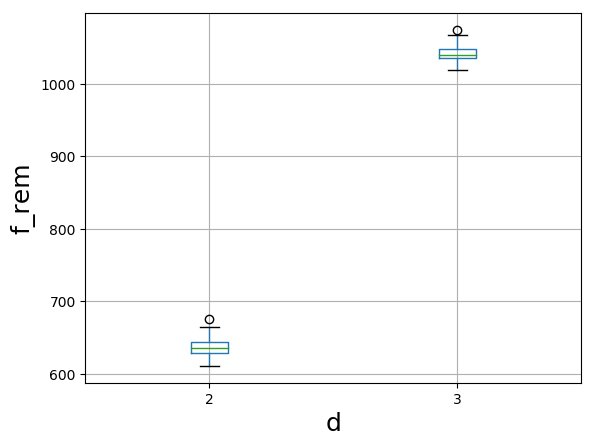
\includegraphics[width=1.2\textwidth]{pictures/med_algo_theo28_comp_rem}
    \end{minipage}
    \hspace*{.8cm}
    \begin{minipage}[t]{.30\textwidth}
        \centering
        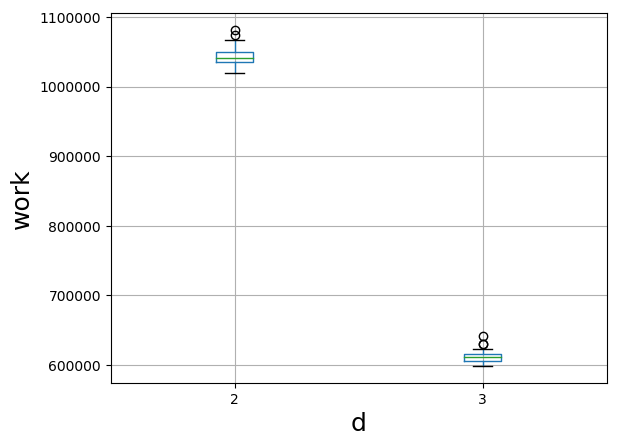
\includegraphics[width=1.25\textwidth]{pictures/med_algo_theo28_comp_work.png}
    \end{minipage}
    \vspace*{-0.1cm}
    \captionof{figure}{Vorhersage und Fit für \fgr sowie die Arbeit $w(n)$.}\label{fig: med_theo28_comp}
\end{figure}

\noindent
Somit ergibt sich ein merklicher Sprung für die \fg aller Elemente, sobald $d(n)$ die nächste Ganzzahl überschreitet. Dies hat direkte Konsequenzen für die Analyse dieser Arbeit, da für die notwendige Parametrisierung nach Theorem~\ref{theo: med_28} bei $k(2^{18}) <3$ sowie $k(2^{19}) \geq 3$ gilt, was das Ergebnis einer Regression verzerrt. Für zukünftige Forschungen wäre es interessant, den Parameter $d(n)$ speziell zu gewichten oder auf bestimmten Intervallen gesondert zu betrachten, was im Rahmen dieser Arbeit zeitlich nicht mehr realisierbar war.
%%%%%%%%%%%%%%%%%%%%%%%%%%%%%%%%%%%%%%%%%%%%%%%%%%%%%%%%%%%%%%%%%
